\scanpage{45}\mspage{44}
\uline{Corollaire} Si $\deleted{\unsure{X}}Y\ll X$, alors \deleted{la relation} toute ombre ouverte d'une \deleted{\unsure{figure|strate de}} \inserted{strate eff.} $Y$ est contenue dans l'ombre ouverte d'une strate de $X$. Plus généralement et par suite, pour tte figure $F$ et \deleted{\unsure{t}} \deleted{sous-figure} \inserted{raffinement} $F'$ de $F$, toute \deleted{strate} \deleted{de ombre ouverte d'une} strate ouverte de $F'$ est contenue dans une (unique) strate ouverte de $F$.

\deleted{\uline{\unsure{Cont|Cond}}. 8 Si \unsure{/}}\enspace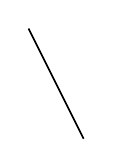
\begin{tikzpicture}[baseline=0pt]\draw[line width=.6pt] (0,.4)--(.7,-1);\end{tikzpicture}

Je viens de m'apercevoir que dans le cas du pseudo disque, \deleted{une} deux lieux disjoints \deleted{\unsure{cq}} \inserted{$x,y$} de l'intérieur (lesquels définissent donc deux ``raffinements'' dudit pseudo-disque), qu'il existe une ``Subdivision'' du disque dont ils soient des \unsure{noeuds|nœuds}. [\uline{NB}. Les \uline{noeuds} d'une figure \inserted{$\deleted{F}F$} sont les multistrates \inserted{de $\deleted{\unsure{X|F}}F$} réduites à un lieu, i.e. les éléments de $F\cap\mathcal L$] Donc \deleted{\unsure{la no}} il n'y a pas lieu de considérer $\{x,y\}$ comme un ``raffinement'', vu qu'il ne s'étend pas en une subdivision. Donc il est inapproprié
